\chapter{Alternative Data Source}
\hrule
\vspace{40pt}

\section{Introduction}

Initially we were not using the Websocket endpoint to gather our data.
Instead we used the Binance historical tick-level orderbook API endpoint.
This returns compressed L2 representations of the orderbook going back multiple years and
for all available trading pairs.
This proved an interesting challenge to parse, so we present our journey here.
This is a cautionary tale, since in the end, we were unable to use this data, so
this chapter also serves as a warning for anyone looking to use this data for a similar application.

\textbf{TL;DR}: This data source has a large amount of missing data.

The data is organized into compressed directories, one for each day. In each directory
there is a snapshot file and an updates file. The snapshot file contains all levels
of the orderbook at the start of the day. See Table \ref{table:snap} \footnote{Originally the raw data was using "b" for bids and "a" for asks in the side column, but we encode bids with $1$s and asks with $0$s so that our data is entirely numerical.}
for an example of a snapshot DataFrame.

\begin{table}[H]
    \centering
    \resizebox{\textwidth}{!}{
        \begin{tabular}{ccccccc}
            \toprule
            Row & timestamp & first\_update\_id & last\_update\_id & side & price & qty \\
            \midrule
            1 & 1689033589005 & 3046269468672 & 3046269468672 & 0 & 30395.5 & 5.174 \\
            2 & 1689033589005 & 3046269468672 & 3046269468672 & 0 & 30395.6 & 0.002 \\
            3 & 1689033589005 & 3046269468672 & 3046269468672 & 0 & 30395.7 & 0.001 \\
            4 & 1689033589005 & 3046269468672 & 3046269468672 & 0 & 30395.8 & 0.001 \\
            \vdots & \vdots & \vdots & \vdots & \vdots & \vdots & \vdots \\
            100343 & 1689033589005 & 3046269468672 & 3046269468672 & 1 & 30395.0 & 0.002 \\
            100344 & 1689033589005 & 3046269468672 & 3046269468672 & 1 & 30395.1 & 0.002 \\
            100345 & 1689033589005 & 3046269468672 & 3046269468672 & 1 & 30395.2 & 0.329 \\
            100346 & 1689033589005 & 3046269468672 & 3046269468672 & 1 & 30395.3 & 0.002 \\
            \bottomrule
        \end{tabular}
    }
    \caption{Example snapshot data for BTCUSDT.}
    \label{table:snap}
\end{table}

The updates file contains all of the updates for the day.
Each row of the updates file represents a change to a price level or a new price level.
So the idea is to start with the snapshot, then iteratively apply the updates, row by row,
to update the state of the orderbook. For example, if a row of the updates table has quantity 0.0,
this means at that time, the corresponding price level cleared and we delete that row
from our reconstructed orderbook. So in this way we can reconstruct the orderbook at any time
by taking our snapshot and applying the updates that happened up to that time.
See Table \ref{table:updates} for an example of an updates DataFrame.



\begin{table*}[ht]
    \centering
    \resizebox{\textwidth}{!}{
        \begin{tabular}{ccccccc}
            \toprule
            Row & timestamp & first\_update\_id & last\_update\_id & side & price & qty \\
            \midrule
            1 & 1689033589005 & 3046269468673 & 3046269468673 & 1 & 30379.8 & 0.24 \\
            2 & 1689033589005 & 3046269468685 & 3046269468685 & 1 & 5000.0 & 0.648 \\
            3 & 1689033589005 & 3046269468690 & 3046269468690 & 0 & 30401.4 & 1.101 \\
            4 & 1689033589005 & 3046269468692 & 3046269468692 & 1 & 30379.9 & 0.0 \\
            \vdots & \vdots & \vdots & \vdots & \vdots & \vdots & \vdots \\
            146793483 & 1689119989003 & 3049606768393 & 3049606768393 & 1 & 5000.0 & 0.534 \\
            146793484 & 1689119989003 & 3049606768394 & 3049606768396 & 1 & 5000.0 & 0.528 \\
            146793485 & 1689119989004 & 3049606768405 & 3049606768405 & 0 & 30618.1 & 3.906 \\
            146793486 & 1689119989004 & 3049606768408 & 3049606768408 & 1 & 5000.0 & 0.53 \\
            \bottomrule
        \end{tabular}
    }
    \caption{Example updates data for BTCUSDT.}
    \label{table:updates}
\end{table*}


\section{On Efficient Parsing}

For our purposes, we want the top $L$ best bids and asks at regular intervals, so
we have to apply the updates to the snapshots for each day and parse this data.
This is non-trivial and took some effort, so we take a small detour here to 
present our parsing algorithm and analyze its efficiency.

This task is harder than one might think on first consideration, due to the fact
that we can't just keep track of the top $L$ levels, since the updates need to be applied
iteratively. For example, if the last price level is cleared and then the $L+1^{\text{th}}$ level
becomes the $L^{\text{th}}$ level, but we were only applying updates to the top $L$ levels,
then this level will not have been correctly updated. For this reason, we must keep track
of the state of the entire orderbook at all times.

Our algorithm initialises the reconstructed orderbook using the snapshot, then iteratively applies
the updates to the reconstructed orderbook. At regular intervals (every $\Delta t$ updates) we
then record the top $L$ best bids and asks from our reconstructed orderbook.

When applying an update, we have three cases that we have to handle:
\begin{enumerate}
    \item A new price level is instantiated.
    \item An existing price level is cleared/deleted.
    \item An existing price level is updated (quantity updated).
\end{enumerate}

For each of these cases, we determine the index in our reconstructed orderbook
where the change needs to happen, then we apply the change. In order to efficiently do this, we split our
orderbook into bids and asks and maintain a sorted ascending order.
This means we can use binary search to find the index which runs in $O(\log_2(S))$ 
where $S$ is the length of the orderbook. Also since most of the updates
happen at the top of the orderbook, if we order the bids/asks so the smallest values
are first (ascending order), then we have a very good average case runtime.
Also for consistency we want the best bid/ask to be first.
Since smaller asks are better, this just means we have to sort our asks in 
ascending order. For bids we have the issue that higher bids are better,
so we could use branching if statements here but this is inefficient for a large
number of iterations, so instead we use a trick. We sort the bids in descending order,
so that the best bid is first, and then we multiply the prices by -1, so that
the smallest values are first. This leads to very fast runtimes in practice.

Once we have found this index, we either insert the update, delete the row or
update an existing row.

Every $\Delta t$ updates, we store the top $L$ best bids and asks from our reconstructed
orderbook in a DataFrame, which is then returned once all the updates
have been applied. Since we know the number of updates and also $\Delta t$, we can
pre-allocated this DataFrame with $\lceil \text{length(updates)} / \Delta t \rceil + 1$ rows\footnote{+1 is for the initial snapshot, t=0 case.}, so that
adding a record is only $O(1)$. 

\section{The Parsing Algorithm}
See Algorithm \ref{algo:levels}.

\begin{algorithm*}
\caption{reconstruct\_orderbook}
\begin{algorithmic}[1]
\Function{reconstruct\_orderbook}{Int $L$, Int $\Delta t$, DataFrame snap, DataFrame updates}
    \State asks $\gets$ snap[side == 0, :]
    \State bids $\gets$ snap[side == 1, :]
    \State sort!(bids, by=price, ascending=false) \Comment{Best bid/ask in first row}
    \State bids[:, price] *= -1.0 \Comment{Trick so we have ascending order}
    \State $N \gets$ $\lceil \text{length(updates)} / \Delta t \rceil+ 1$ \Comment{+ 1 for initial snapshot row}
    \State top\_bids $\gets$ bids[1:L, :] \Comment{Initial case}
    \State top\_asks $\gets$ asks[1:L, :]
    \State levels $\gets$ zeros($N$, $1 + 4L$)  \Comment{Pre-allocate our parsed levels}
    \State levels[1, :] $\gets$ concat([ \Comment{Initial edge case} \\
    \hspace{35pt}  snap[1, timestamp], \\
    \hspace{35pt}  top\_bids[:, price] * -1.0, \\
    \hspace{35pt}  top\_asks[:, price],\\
    \hspace{35pt}  top\_bids[:, qty],\\
    \hspace{35pt}  top\_asks[:, qty]\\
    \hspace{16pt}])
    \State levels\_idx $\gets 2$
    \For{(t, update) in \text{enumerate}(updates)} \Comment{Iterate over each row of updates}
        \If{update.side == 1}
            \State orderbook $\gets$ bids  \Comment{orderbook is a reference not a copy}
            \State update.price *= -1  \Comment{Trick so we have descending order}
        \Else
            \State orderbook $\gets$ asks
        \EndIf
        \State insert\_idx $\gets$ searchsortedfirst(orderbook[:, price], update.price)
        \If{insert\_idx $>$ nrow(orderbook) or orderbook[insert\_idx, price] $\neq$ update.price}
            \State insert!(orderbook, insert\_idx, update) \Comment{Case 1: New price}
            \ElsIf{update.qty $== 0.0$} \Comment{Case 2: Deleting a price}
            \State deleteat!(orderbook, insert\_idx)

            \Else  \Comment{Case 3: Updating the quantity for a price}             
            \State orderbook[insert\_idx, :] $\gets$ update
        \EndIf \\

        
        \If{$t ~ \% ~ \Delta t == 0$} \Comment{Record the state of the top L levels every $\Delta t$ updates.}
            \State top\_bids $\gets$ bids[1:L, :]
            \State top\_asks $\gets$ asks[1:L, :]
            \State levels[levels\_idx, :] $\gets$ concat([ \\
            \hspace{65pt}    update.timestamp, \\
            \hspace{65pt}  top\_bids[:, price] * -1.0, \\
            \hspace{65pt}  top\_asks[:, price],\\
            \hspace{65pt}  top\_bids[:, qty],\\
            \hspace{65pt}  top\_asks[:, qty]\\
            \hspace{47pt}])
            \State levels\_idx += 1
        \EndIf
    \EndFor
    \State \Return levels
\EndFunction
\end{algorithmic}
\label{algo:levels}
\end{algorithm*}

\section{Complexity Analysis}

If we denote $U$ to be the number of updates and $S$ to be the size of the initial snapshot/number of levels
in our reconstructed orderbook (on average this should be roughly constant). Then we see that 
Algorithm \ref{algo:levels} has $O(US)$ worse case runtime complexity, since for each of the $U$ 
updates, we searchsorted through our reconstructed orderbook, which runs in $O(\log_2(S))$ worst case,
and then either delete, insert or update a price level. Inserting and deleting are both $O(S)$ worst case,
but updating is only $O(1)$, so worst case we have $O(\log_2(S) + S) = O(S)$  time complexity per
iteration. So in total we have $O(US)$ worst case time complexity. Then we also have $O(U + S)$ memory
complexity since we store the updates and reconstructed orderbook in memory at all times. 
In practice we can use a RecordCursor object to efficiently read the updates line by line, instead
of having to load them into memory all at once. This reduces the memory complexity down to $O(S)$.

Note that $U \gg S$ and so for efficiency we mostly care about the complexities in terms of $U$. 
For our data we observe $U \approx 1.5 \times 10^3 S$.

So we see that we achieve linear worst case time complexity in $U$ and, due to the
sequential nature of the updates, this is clearly the best possible time complexity for 
this problem. We verify the linear time complexity experimentally in Figure \ref{complexity}


\section{Data Issues}

We can apply our algorithm to each day of data and then combine the results.
In order to check our data, we parse the data for several months in 2023 of BTCUSDT data 
and then compare to a reference.
For our reference, we have access to hourly BTCUSDT mid-prices from an undisclosed source,
going back 1 year.
We resample our parsed data to an hourly resolution and then calculate hourly mid-prices.
We plot our parsed data against the reference data in Figure \ref{missing}.

Unfortunately we find that there is a lot of missing data and we verify that this
is from the underlying raw data and not an issue with our parsing.
Due to this, we are unable to use this historical data for our purposes.

\begin{figure}[htpb]
    \centering
    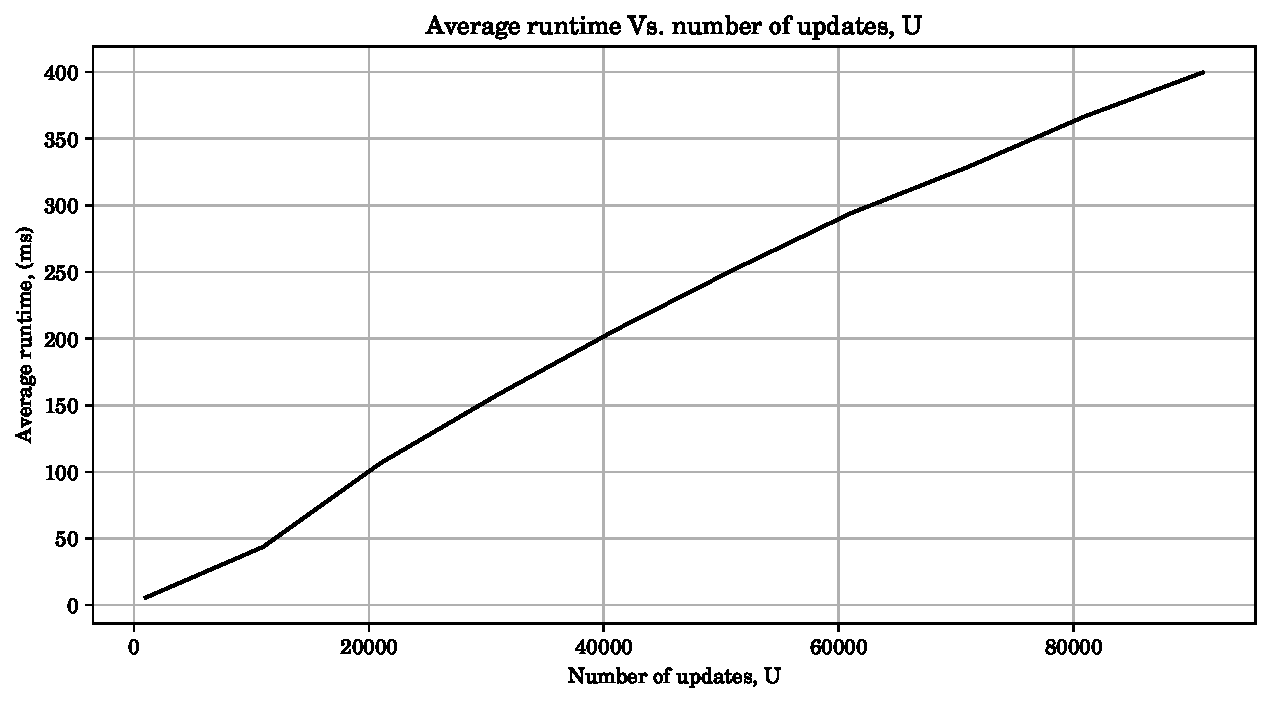
\includegraphics[width=1.0\textwidth]{./images/complexity.pdf}
    \caption{reconstruct\_orderbook runtime as a function of the number of updates, $U$.\\ Note that the runtimes are recorded 100 times and then averaged.}
    \label{complexity}
\end{figure}

\begin{figure}[htpb]
    \centering
    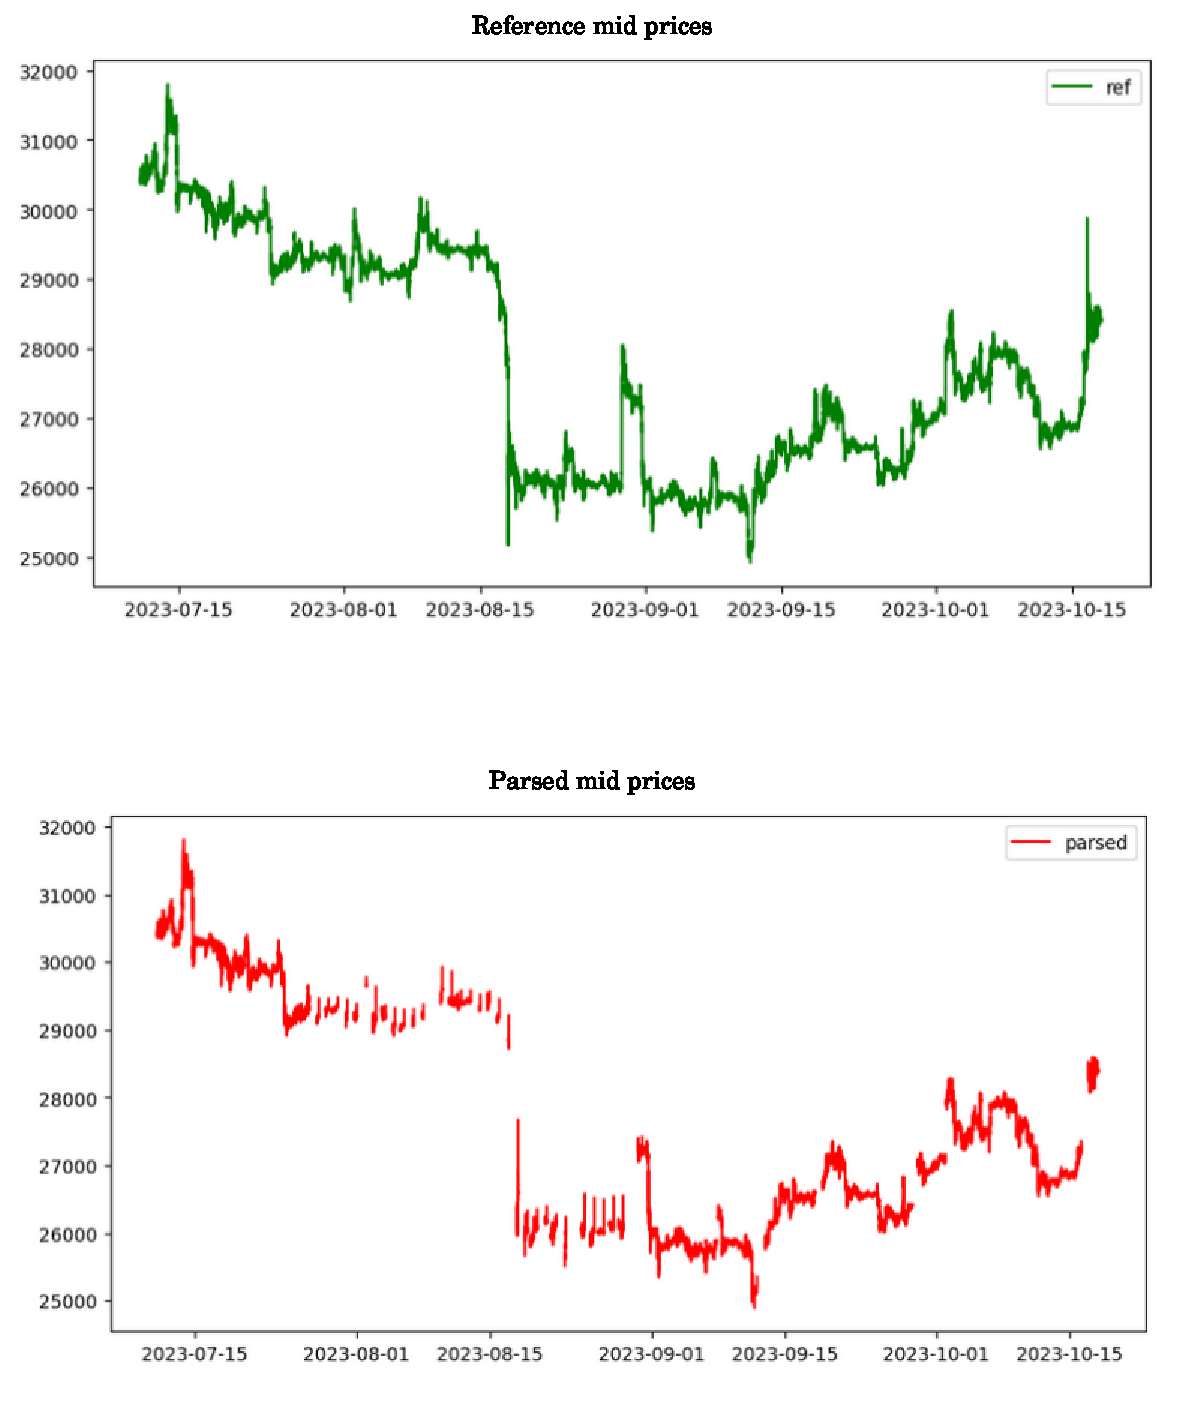
\includegraphics[width=1.0\textwidth]{./images/stitched.pdf}
    \caption{Reference hourly mid-prices (top) Vs. parsed mid-prices (bottom). Observe the general shape is correct, however
    there are large irregular gaps due to missing data.}
    \label{missing}
\end{figure}
